% Ontology of the knowledge graph (representasi.md section 5; system/ontology/ontology.ttl).
% Compile: pdflatex ontologi.tex  (standalone; \input the tikzpicture in the paper)
\documentclass[tikz,border=4pt]{standalone}
\usetikzlibrary{positioning,arrows.meta,fit}
\begin{document}
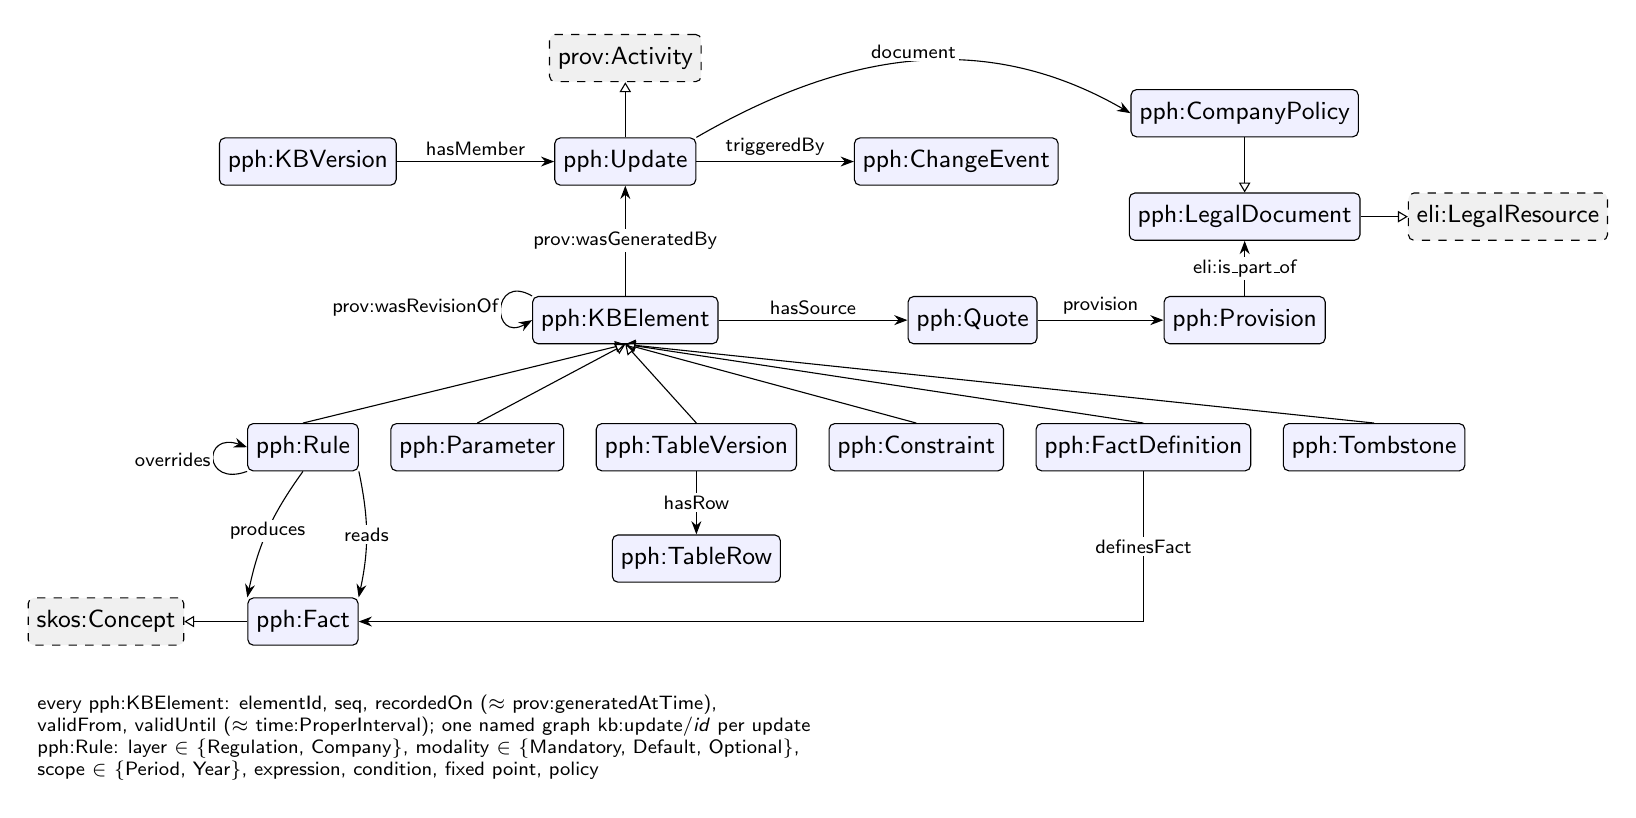
\begin{tikzpicture}[
  node distance=7mm and 9mm,
  cls/.style={draw,rounded corners=2pt,fill=blue!6,font=\small\sffamily,minimum height=6mm,inner sep=3pt},
  ext/.style={cls,fill=gray!12,dashed},
  sub/.style={-{Triangle[open]},thin},
  rel/.style={-{Stealth},thin},
  lab/.style={font=\scriptsize\sffamily,fill=white,inner sep=1pt}]

% knowledge base elements
\node[cls] (el) {pph:KBElement};
\node[cls,below left=10mm and 22mm of el] (rule) {pph:Rule};
\node[cls,right=4mm of rule] (par) {pph:Parameter};
\node[cls,right=4mm of par] (tab) {pph:TableVersion};
\node[cls,right=4mm of tab] (con) {pph:Constraint};
\node[cls,right=4mm of con] (fd) {pph:FactDefinition};
\node[cls,right=4mm of fd] (tomb) {pph:Tombstone};
\foreach \n in {rule,par,tab,con,fd,tomb} \draw[sub] (\n.north) -- (el.south);
\node[cls,below=8mm of tab] (row) {pph:TableRow};
\draw[rel] (tab) -- node[lab]{hasRow} (row);

% facts
\node[cls,below=16mm of rule] (fact) {pph:Fact};
\node[ext,left=8mm of fact] (concept) {skos:Concept};
\draw[sub] (fact) -- (concept);
\draw[rel] (rule.south) to[bend right=12] node[lab]{produces} (fact.north west);
\draw[rel] (rule.south east) to[bend left=12] node[lab]{reads} (fact.north east);
\draw[rel] (fd.south) |- node[lab,pos=0.25]{definesFact} (fact.east);
\draw[rel] (rule.south west) to[out=200,in=160,looseness=5] node[lab,left]{overrides} (rule.west);

% provenance
\node[cls,right=24mm of el] (quote) {pph:Quote};
\node[cls,right=16mm of quote] (prov) {pph:Provision};
\node[cls,above=7mm of prov] (doc) {pph:LegalDocument};
\node[ext,right=6mm of doc] (eli) {eli:LegalResource};
\node[cls,above=7mm of doc] (pol) {pph:CompanyPolicy};
\draw[rel] (el) -- node[lab,above=1pt]{hasSource} (quote);
\draw[rel] (quote) -- node[lab,above=1pt]{provision} (prov);
\draw[rel] (prov) -- node[lab]{eli:is\_part\_of} (doc);
\draw[sub] (doc) -- (eli);
\draw[sub] (pol) -- (doc);

% change and versions
\node[cls,above=14mm of el] (upd) {pph:Update};
\node[cls,left=20mm of upd] (ver) {pph:KBVersion};
\node[cls,right=20mm of upd] (ev) {pph:ChangeEvent};
\node[ext,above=7mm of upd] (act) {prov:Activity};
\draw[rel] (el) -- node[lab]{prov:wasGeneratedBy} (upd);
\draw[rel] (ver) -- node[lab,above=1pt]{hasMember} (upd);
\draw[rel] (upd) -- node[lab,above=1pt]{triggeredBy} (ev);
\draw[sub] (upd) -- (act);
\draw[rel] (upd.north east) to[out=30,in=150] node[lab,above]{document} (pol.west);
\draw[rel] (el.north west) to[out=150,in=210,looseness=5] node[lab,left]{prov:wasRevisionOf} (el.west);

\node[font=\scriptsize\sffamily,align=left,anchor=north west] at ([yshift=-5mm]concept.south west)
  {every pph:KBElement: elementId, seq, recordedOn ($\approx$ prov:generatedAtTime),\\
   validFrom, validUntil ($\approx$ time:ProperInterval); one named graph kb:update/\textit{id} per update\\
   pph:Rule: layer $\in$ \{Regulation, Company\}, modality $\in$ \{Mandatory, Default, Optional\},\\
   scope $\in$ \{Period, Year\}, expression, condition, fixed point, policy};
\end{tikzpicture}
\end{document}
